\section{INTRODUCTION \hrulefill}

The purpose of the project is to make an intuitive and powerful bioinformatics
search engine which provides online access to a large dataset of protein
isoelectric points which has been compiled by Aston University researchers and
students over the course of several years.

\subsection{Background}
Bioinformatics is a multidisciplinary field which uses computational methods to
aid in biological research by creating systems for storing, organising and
analysing complex biological data. Within this field there are many online
databases categorising biological information at the molecular level, and one
such purpose of these is for storing the functional and physical properties of
proteins. Currently, no such database exists for one of the most widely-used,
important, and useful properties of proteins: the isoelectric point (pI). An
isoelectric point is the acidity (pH) at which a molecule carries no net charge;
below the isoelectric point, proteins have a net positive charge, above it a net
negative charge. Additionally, proteins are at their lowest solubility at their
isoelectric point, and this makes the isoelectric point a vitally important
property when both characterising and purifying proteins.

The dataset which has been compiled is a collection of entries stored as a
non-relational table, and for each entry it records the name of the protein, its
identity, origin, experimental conditions, its isoelectric point, and other
pertinent data. There are also links to a heterogeneous collection of databases
containing associated data, such as amino acid sequence, function, etc. A
website that warehouses this data and offers a robust and adaptable GUI for
searching, viewing and downloading results would greatly increase the
accessibility of the dataset.

\subsection{Objectives}

\begin{enumerate}
\item To build a free (as in freedom) web application for searching and viewing
  protein isoelectric points.
\item To produce a bioinformatics tool with real world value for future
  scientific research.
\item The application should provide intuitive but powerful searching
  facilities.
\item The application should provide a convenient means for a certified user to
  edit and upload additional data.
\item The application should present information in a usable and efficient form.
\item Users should be allowed to download generated results for offline use.
\item Adequate security precautions should be taken to minimise the risk of data
  being sabotaged or stolen.
\item The implementation should use a clean model view controller architecture.
\item Comprehensive test coverage of the API and common use cases should be
  automated.
\item The application should be scalable for much larger datasets.
\end{enumerate}

\subsection{Deliverables}
Two primary deliverables can be derived from the project objectives:

\begin{enumerate}
\item An updatable relational database warehousing the provided dataset.
\item A web-accessible GUI with searching and downloading functionality.
\end{enumerate}

\noindent
Additionally, two further deliverables can be derived from the same requirements
document as secondary features:

\begin{enumerate}
\item A web-accessible GUI to support editing and uploading new data.
\item Support for NCBI BLAST protein sequence matching \cite{NCBIND}.
\end{enumerate}

\subsection{Required Resources}
The deliverable product for this product is a website that offers a publicly
available service. To this end, there are three required resources:

\begin{enumerate}
\item A server which can be host the website and process and respond to requests
  from clients.
\item A public IP address which this server can be assigned to for external
  access.
\item A domain name which will resolve to this IP address.
\end{enumerate}

Additional stipulations for the requirements are that the server should use a
GNU/Linux operating system so as to support most common webserver stacks, and
that it should be a dedicated physical machine with root access so as to allow
for more involved configuration and testing. Assuming that the University can
supply the webserver and access to one of its IP addresses, the budget for the
project need only cover the cost of domain registration, which is very cheap
(less than \pounds20 per year).

\subsection{Required Technologies}
There are an almost immeasurable number of web technologies that offer the
functionality required to implement this project. From a time-management
perspective, one of the main priorities for the work undertaken in the first
term is to research these existing technologies, and to gain a better
understanding of the strengths of each in order to select an appropriate choice
for the implementation of the final product. Figure \ref{fig:flow-tech-choices}
shows the process by which these choices are made, starting off with the
highest-level decision (the choice of paradigms: whether it be a client-server
model, a distributed network application, the format for data transmission etc.)
and increasing in granularity down to the lowest-level choice of individual
frameworks and libraries. Each decision is not immutable, and previous decisions
may be re-evaluated over time in an iterative fashion. This is to encourage
implementation work to begin at an early stage in order to produce a functioning
prototype, without the need to have performed a depth first analysis of every
possible technology which could be used. Work on the implementation can begin
once the programming language(s) have been decided upon, so it is important to
reach a decision upon this as early into TP1 as is possible, although this
decision is free to change over the course of the project, providing there is a
realistic justification for this change and adequate time to re-implement any
existing functionality.

\begin{figure}[H]
\centering
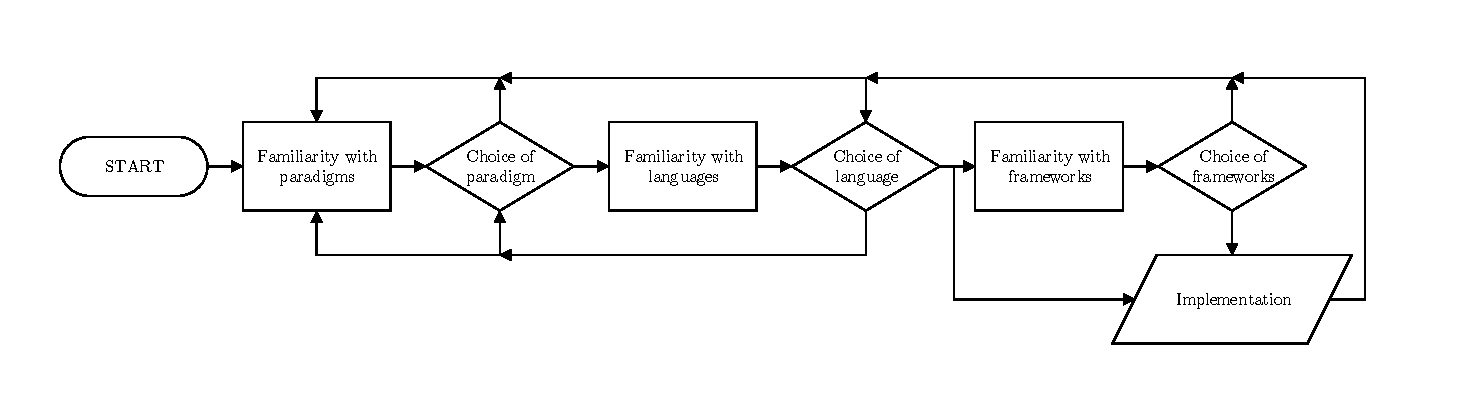
\includegraphics[width=7.2in]{assets/flow-tech-choices.pdf}
\caption{A diagrammatic view of the process of adopting technologies}
\label{fig:flow-tech-choices}
\end{figure}

\newpage
\subsection{Required Skills}
This technically ambitious project will require the adoption of a number of new
skillsets, a brief overview of which is included below:

\subsubsection{Project management}

\begin{enumerate}
\item Single-developer project management - including good communication with
  clients and stakeholders, selecting an appropriate software development
  process, setting realistic deadlines and goals, and tracking the progress of a
  long term development project.
\item Working with a mature codebase - this includes proper version control and
  use of a sane branching model, and documenting decisions and all source code
  throughout the duration of development.
\item Maintenance and tooling - developing a software product with long-term
  usability as a primary goal, as well as appropriate documentation to allow
  other developers to administrate the website.
\item Software quality - appropriate use of issue trackers and bug ticketing to
  track the lifecycle of implementation bugs and regressions, and adopting a
  meaningful release cycle and version numbering scheme.
\end{enumerate}

\subsubsection{Back-end development}

\begin{enumerate}
\setcounter{enumi}{4}
\item Relational data modelling and database design - designing and formalising
  database schemas, and providing advanced querying functionality.
\item Computing with large datasets - appropriately using existing tools and
  software patterns for working with large persistent data models.
\item Performance optimising - server-side optimisations to enable high
  performance serving of web pages such as caching, and successful cache
  invalidation techniques for the webserver and database.
\item Designing secure web applications - using formal and established methods
  to ensure data integrity of critical biological research data.
\end{enumerate}

\subsubsection{Front-end development}
\begin{enumerate}
\setcounter{enumi}{8}
\item User interface design - working with clients to design accessible and
  easy-to-user GUIs, including appropriate use of Human Computer Interaction
  techniques and user testing.
\item Responsive website design - correctly using HTML5 and CSS3 features to
  allow for site accessibility from a wide range of different devices.
\item Client-side scripting - using mobile code such as JavaScript to enrich
  user interfaces using technologies such as AJAX and dynamic content generation
  and control.
\end{enumerate}
